\section{Consuntivo}

\subsection{\ARM}

La differenza di ore da quelle preventivate nella sezione 4 di questo documento a quelle effettivamente fatte è la seguente:

\begin{table}[h]
	\begin{center}
		\begin{tabular}{|c|c|c|c|c|}
			\hline
			\textbf{Ruolo}	& \textbf{Ore Preventivate} & \textbf{Differenza ore} & \textbf{Costo} & \textbf{Differenza costo}\\
			\hline
			\Pm &	26  &	-6 &	780 &	-180\\
			\hline
			\Am	&	20 &	-1 & 400 & -20\\
			\hline
			\An		&	73 &	+2 & 1825 & +50\\
			\hline
			\Ver	&	56 &	+9 & 840 & +135\\
			\hline
			\textbf{totale}	&	\textbf{175} &	\textbf{+4} & \textbf{3845} & \textbf{-15}\\
			\hline
		\end{tabular}
	\end{center}
	\caption{Consuntivo \ARM}
\end{table}

Ed il lavoro risulta essere così partizionato:

\begin{figure}[H]
	\centering 
	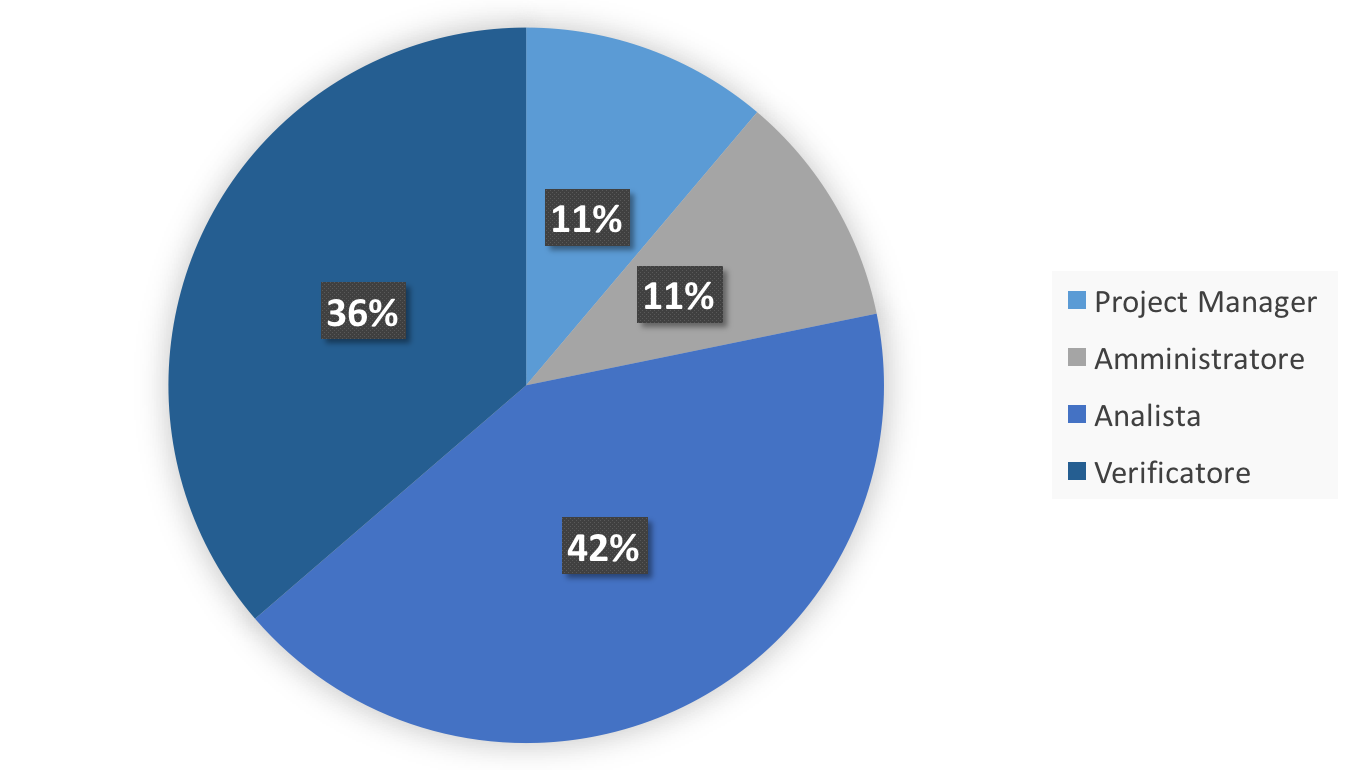
\includegraphics[scale=0.7]{Immagini/Consuntivo/GraficoConsuntivo.png}
	\caption{Consuntivo delle ore per ruolo, \ARM}
\end{figure}

Dal consuntivo, dunque, emerge un \textbf{risparmio di 15 euro} rispetto ai costi preventivati in precedenza.

\newpage

\subsection{\ARD}
La differenza di ore da quelle preventivate nella sezione 4 di questo documento a quelle effettivamente fatte è la seguente:

\begin{table}[h]
	\begin{center}
		\begin{tabular}{|c|c|c|c|c|}
			\hline
			\textbf{Ruolo}	& \textbf{Ore Preventivate} & \textbf{Differenza ore} & \textbf{Costo} & \textbf{Differenza costo}\\
			\hline
			\Pm &	5  & -2 & 150 & 60	\\
			\hline
			\Am	&	5 & -2 & 100 & 40\\
			\hline
			\An	&	18 & +12 & 450 & 300\\
			\hline
			\Ver &	11 & +3 & 165 & 45\\
			\hline
			\textbf{totale}	&	\textbf{39} & \textbf{+11} & \textbf{865} & \textbf{+445}\\
			\hline
		\end{tabular}
	\end{center}
	\caption{Consuntivo \ARD}
\end{table}

Ed il lavoro risulta essere così partizionato:

\begin{figure}[H]
	\centering 
	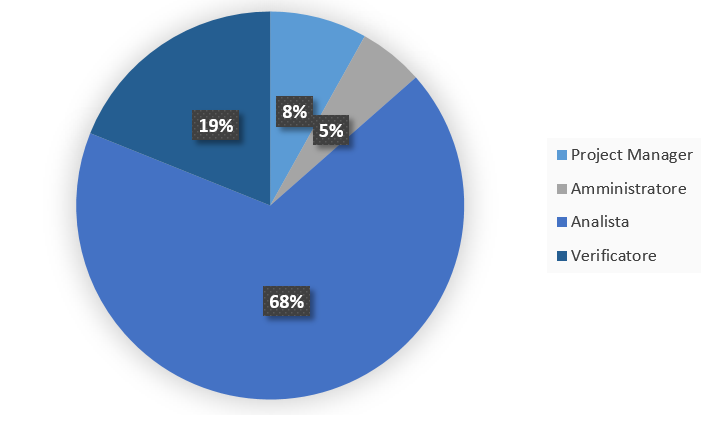
\includegraphics[scale=1.25]{Immagini/Consuntivo/ConsuntivoARD.png}
	\caption{Consuntivo delle ore per ruolo, \ARD}
\end{figure}

Dal consuntivo, dunque, emerge un \textbf{eccesso di 445 euro} rispetto ai costi preventivati in precedenza.

\newpage

\subsection{\PA}
La differenza di ore da quelle preventivate nella sezione 4 di questo documento a quelle effettivamente fatte è la seguente:

\begin{table}[h]
	\begin{center}
		\begin{tabular}{|c|c|c|c|c|}
			\hline
			\textbf{Ruolo}	& \textbf{Ore Preventivate} & \textbf{Differenza ore} & \textbf{Costo} & \textbf{Differenza costo}\\
			\hline
			\Pm &	6  & 0 &	180 & 0	\\
			\hline
			\Am	&	6 &	-1 & 160 & -60\\
			\hline
			\Prog	&	129 & -9 & 2838 & -198\\
			\hline
			\Ver &	62 & +3 & 930 & +45\\
			\hline
			\textbf{totale}	&	\textbf{203} & \textbf{-7} & \textbf{4108} & \textbf{-213}\\
			\hline
		\end{tabular}
	\end{center}
	\caption{Consuntivo \PA}
\end{table}

\begin{figure}[H]
	\centering 
	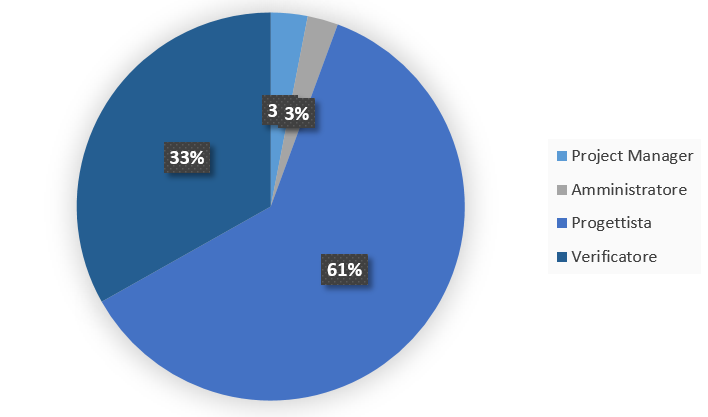
\includegraphics[scale=1.25]{Immagini/Consuntivo/ConsuntivoPA.png}
	\caption{Consuntivo delle ore per ruolo, \PA}
\end{figure}

Dal consuntivo, dunque, emerge un \textbf{risparmio di 213 euro} rispetto ai costi preventivati in precedenza.

\newpage

\subsection{\PD}
La differenza di ore da quelle preventivate nella sezione 4 di questo documento a quelle effettivamente fatte è la seguente:


\begin{table}[h]
	\begin{center}
		\begin{tabular}{|c|c|c|c|c|}
			\hline
			\textbf{Ruolo}	& \textbf{Ore Preventivate} & \textbf{Differenza ore} & \textbf{Costo} & \textbf{Differenza costo}\\
			\hline
			\Pm &	7  & 0 &	210 &	0\\
			\hline
			\Am	&	7 &	0 & 140 & 0\\
			\hline
			\Prog	&	76 & -11 & 1672 & -242 \\
			\hline
			\Ver &	38 & +4 & 570 & +60\\
			\hline
			\textbf{totale}	&	\textbf{128} & \textbf{-7} & \textbf{2592} & \textbf{-182} \\
			\hline
		\end{tabular}
	\end{center}
	\caption{Consuntivo \PD}
\end{table}

\begin{figure}[H]
	\centering 
	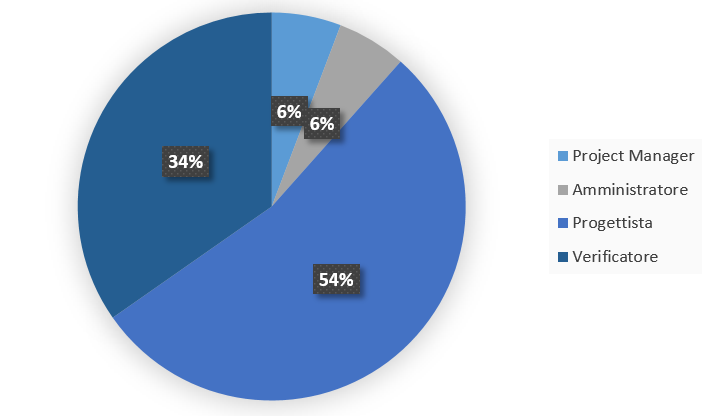
\includegraphics[scale=1.25]{Immagini/Consuntivo/ConsuntivoPD.png}
	\caption{Consuntivo delle ore per ruolo, \PD}
\end{figure}

Dal consuntivo, dunque, emerge un \textbf{risparmio di 182 euro} rispetto ai costi preventivati in precedenza.
